\chapter{Réalisation et Tests}

\section{Introduction}
Ce chapitre aborde la concrétisation de la plateforme d'orchestration Cyber Threat Intelligence (Cyber-HUD). Après avoir défini l'architecture et les spécifications de notre solution, nous détaillerons ici les aspects techniques de son implémentation. L'objectif est de démontrer comment les différents modules (Pipeline CTI, Pipeline Telegram, Backend, Frontend et Authentification) s'intègrent pour former une solution SOC unifiée, performante et sécurisée. Enfin, nous présenterons les résultats des tests de validation confirmant la robustesse du système.

\section{Implémentation du système d'authentification (Keycloak)}

\subsection{Configuration du Realm et des clients Keycloak}
La sécurisation de la plateforme repose sur \textbf{Keycloak}, une solution open source de gestion des identités et des accès (IAM). Un Realm dédié (\texttt{CyberHUD}) a été configuré via un script de provisioning automatisé. Deux clients ont été créés : un client frontend (React) pour l'authentification publique et un client backend (FastAPI) pour valider les tokens.

\subsection{Intégration OpenID Connect / tokens JWT (RS256) dans FastAPI}
Le backend FastAPI a été sécurisé en intégrant le protocole \textbf{OpenID Connect (OIDC)}. Lorsqu'un utilisateur s'authentifie, Keycloak génère un \textbf{JSON Web Token (JWT)} signé avec l'algorithme asymétrique \textbf{RS256}. L'API FastAPI intercepte chaque requête, extrait le JWT du header d'autorisation et le valide en s'assurant de son intégrité via les clés publiques de Keycloak.

\subsection{Mise en place du RBAC (rôles admin / analyste)}
La gestion des accès est basée sur le modèle \textbf{RBAC (Role-Based Access Control)}. Le backend vérifie les rôles inclus dans le payload du token JWT pour accorder ou refuser l'accès aux différents endpoints.

\subsection{Résultat : Interface de connexion et Dashboard différencié}
L'application affiche une page de connexion moderne et sécurisée gérée par Keycloak. L'accès est validé pour le compte Administrateur (\texttt{admin\_cti}).

% Forcer le compteur de figure à commencer à 9 pour la première figure de cette section
\setcounter{figure}{8}

\begin{figure}[H]
    \centering
    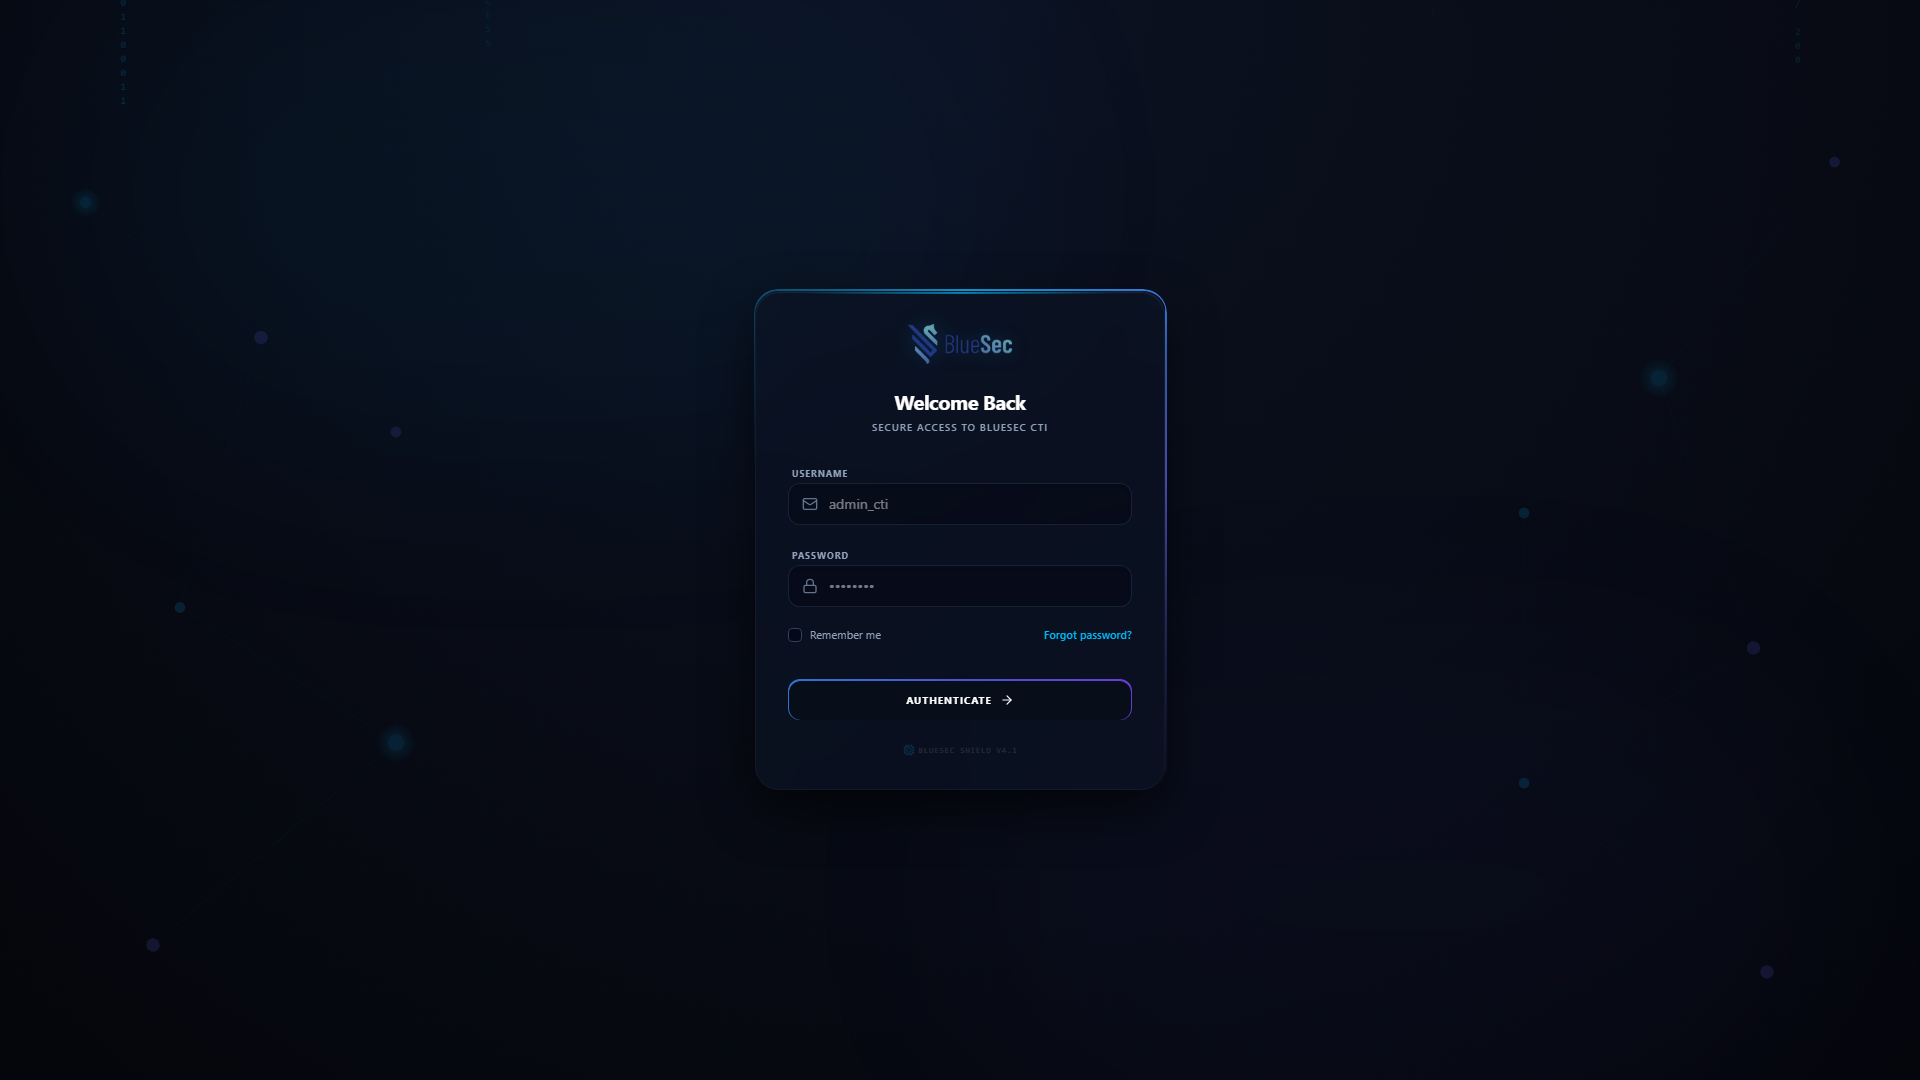
\includegraphics[width=0.8\textwidth]{screenshot/09_page_connexion.png}
    \caption{Interface de connexion Keycloak (Authentification du compte Administrateur)}
    \label{fig:login}
\end{figure}

\begin{figure}[H]
    \centering
    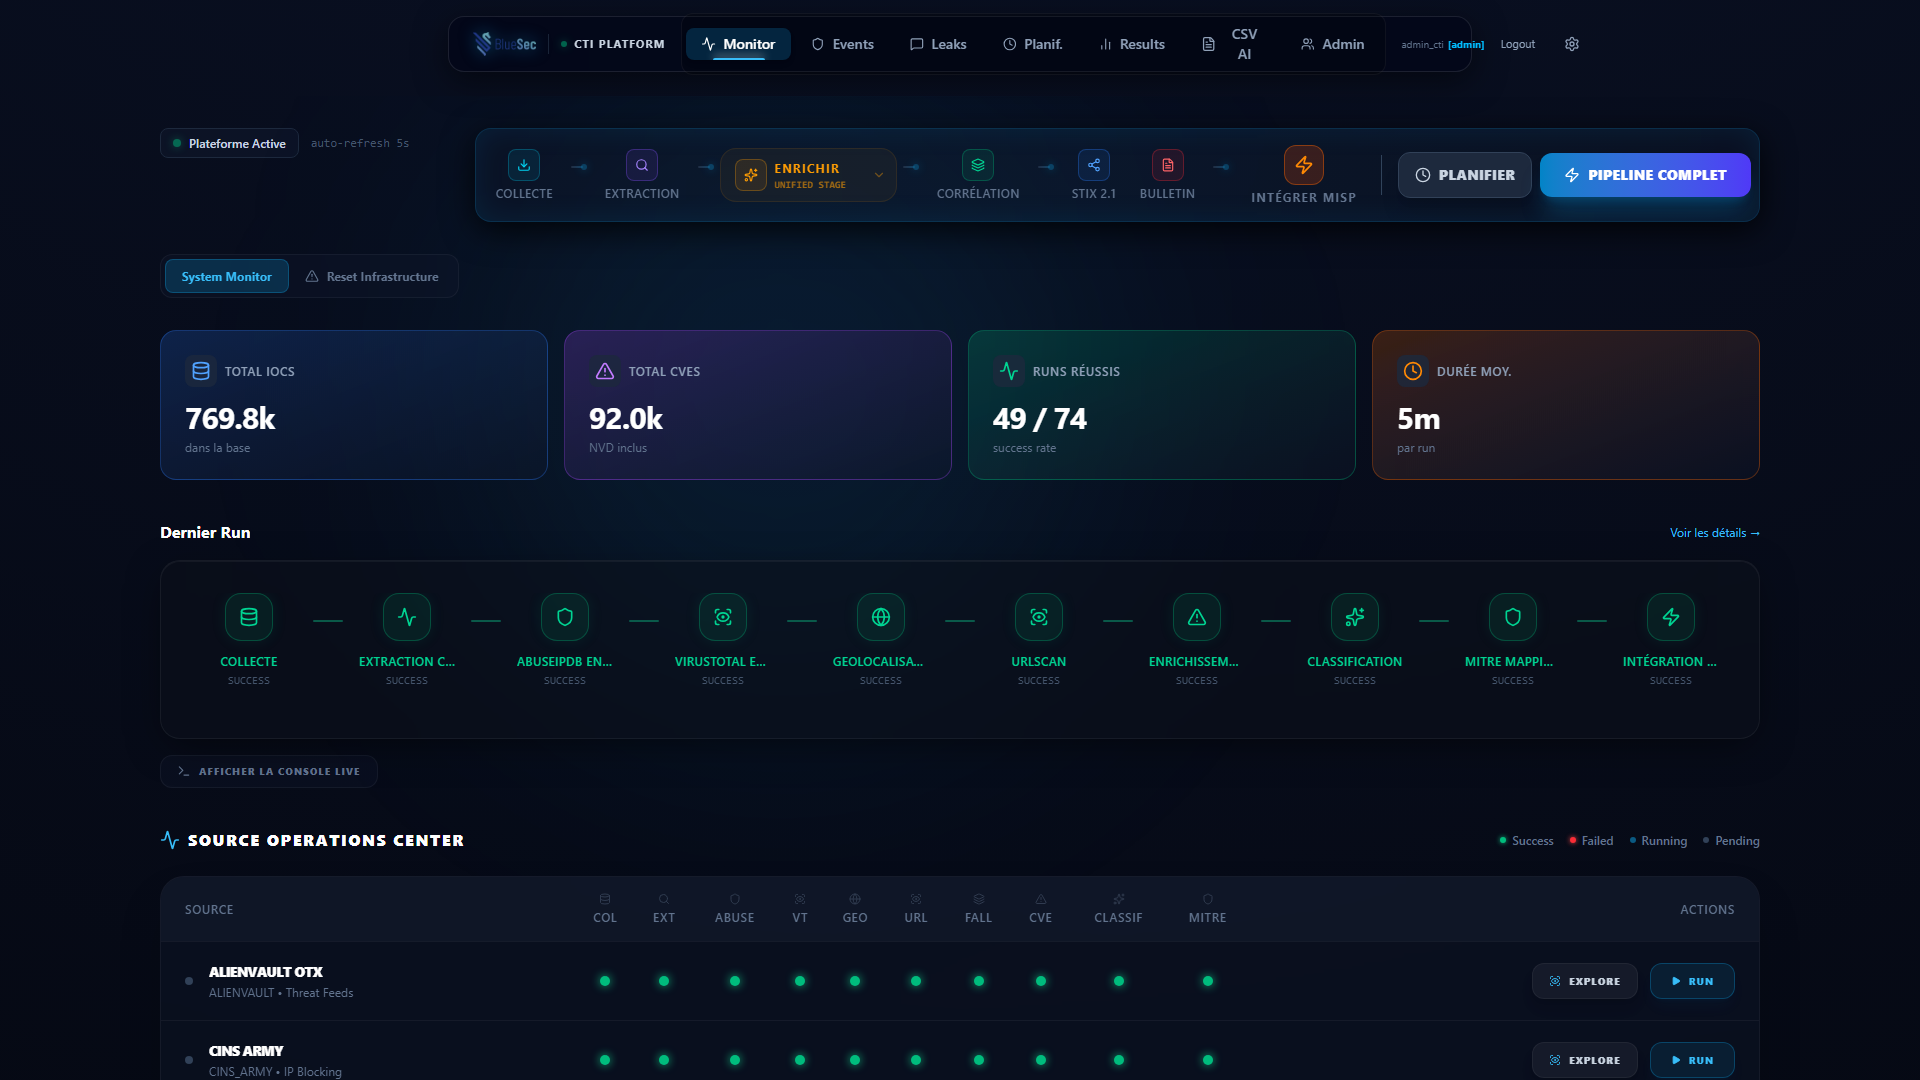
\includegraphics[width=0.9\textwidth]{screenshot/10_dashboard_principal.png}
    \caption{Dashboard principal SOC présentant les statistiques globales et télémétries}
    \label{fig:dashboard}
\end{figure}

\section{Implémentation du Pipeline IOC/CVE (Pipeline 1)}

\subsection{Collecte et Extraction multi-sources}
Le script se charge de récupérer de manière asynchrone les données brutes provenant de sources CTI réputées (AlienVault, NVD, Abuse.ch, etc.). Les données brutes collectées sont traitées par le dossier \texttt{extraction\_ioc\_cve}. Des Regex avancées et un filtrage par "Whitelist" garantissent une extraction de haute fidélité des éléments tels que : \textbf{Adresses IP, Domaines, URL, Hashs et CVEs}.

\subsection{Enrichissement multi-couches et Scoring}
Les IOC passent par le processus d'enrichissement s'interfaçant avec AbuseIPDB, URLScan.io, et VirusTotal. Un système de géolocalisation ultra-rapide a été implémenté (< 1ms par IP). Un algorithme de scoring calcule un niveau de risque global pour chaque indicateur pour prioriser les menaces.

\subsection{Mapping MITRE ATT\&CK et Intégration MISP}
Les IOC enrichis sont classifiés via un mappage NLP, corrélant les comportements avec les tactiques et techniques \textbf{MITRE ATT\&CK}. Enfin, les données sont normalisées au format standard \textbf{STIX 2.1} et poussées vers MISP via son API REST.

\begin{figure}[H]
    \centering
    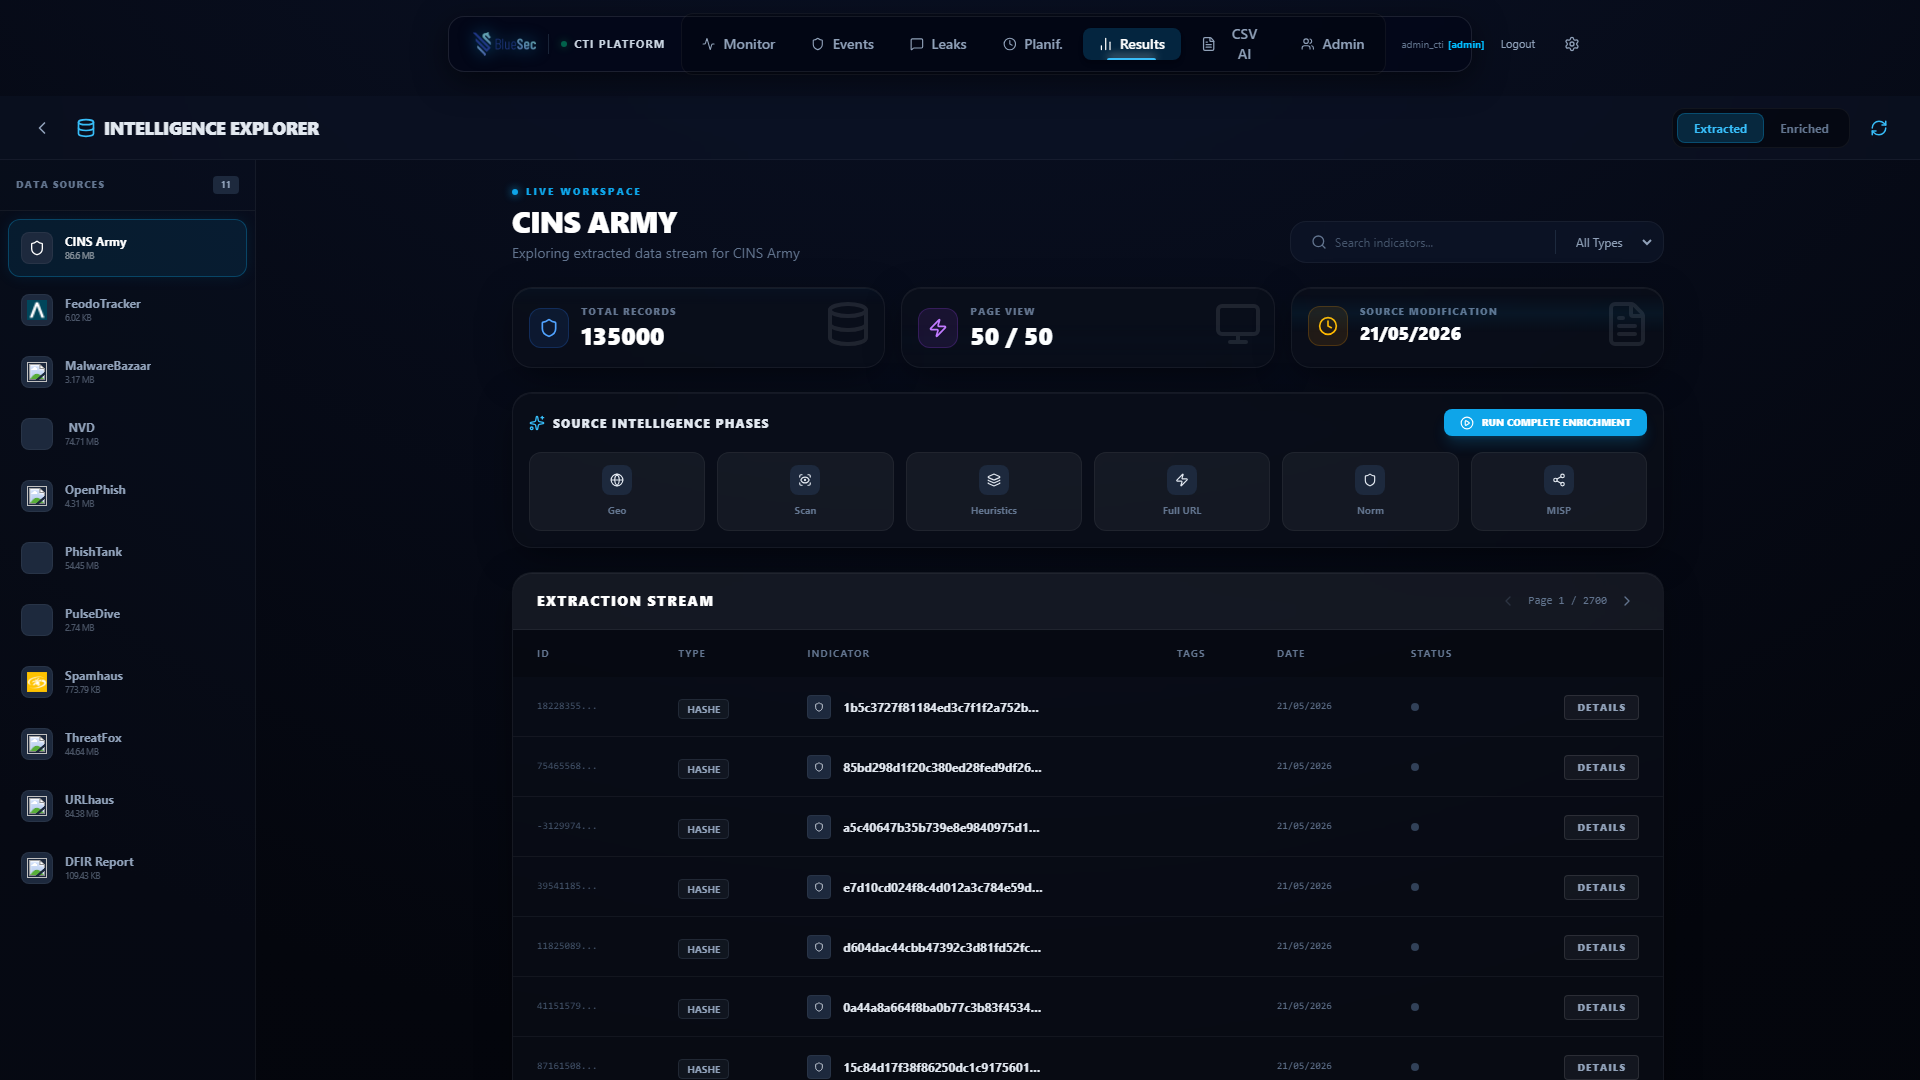
\includegraphics[width=0.9\textwidth]{screenshot/11_page_ioc_cve.png}
    \caption{Interface de visualisation et de filtrage détaillé des IOC et CVE extraits}
    \label{fig:ioc_cve}
\end{figure}

\section{Implémentation du Pipeline Telegram (Pipeline 2)}

\subsection{Collecteur Telegram et Analyse sémantique LLM}
Le pipeline "Threat Leak Intelligence" utilise \textbf{Telethon} pour "crawler" les canaux cibles. Les fichiers joints suspects (CSV, SQL, XLSX) et les textes sont transmis à un module IA basé sur \textbf{LangChain} et un LLM pour la classification (Credentials, BDD, etc.), l'évaluation de sévérité, et l'élimination des faux positifs.

\subsection{Corrélation et Génération de bulletins}
Le système consolide quotidiennement les incidents extraits. Il emploie une corrélation sémantique en double-passe pour regrouper les mentions multiples. Le résultat est converti en un rapport PDF professionnel "BlueSec".

\begin{figure}[H]
    \centering
    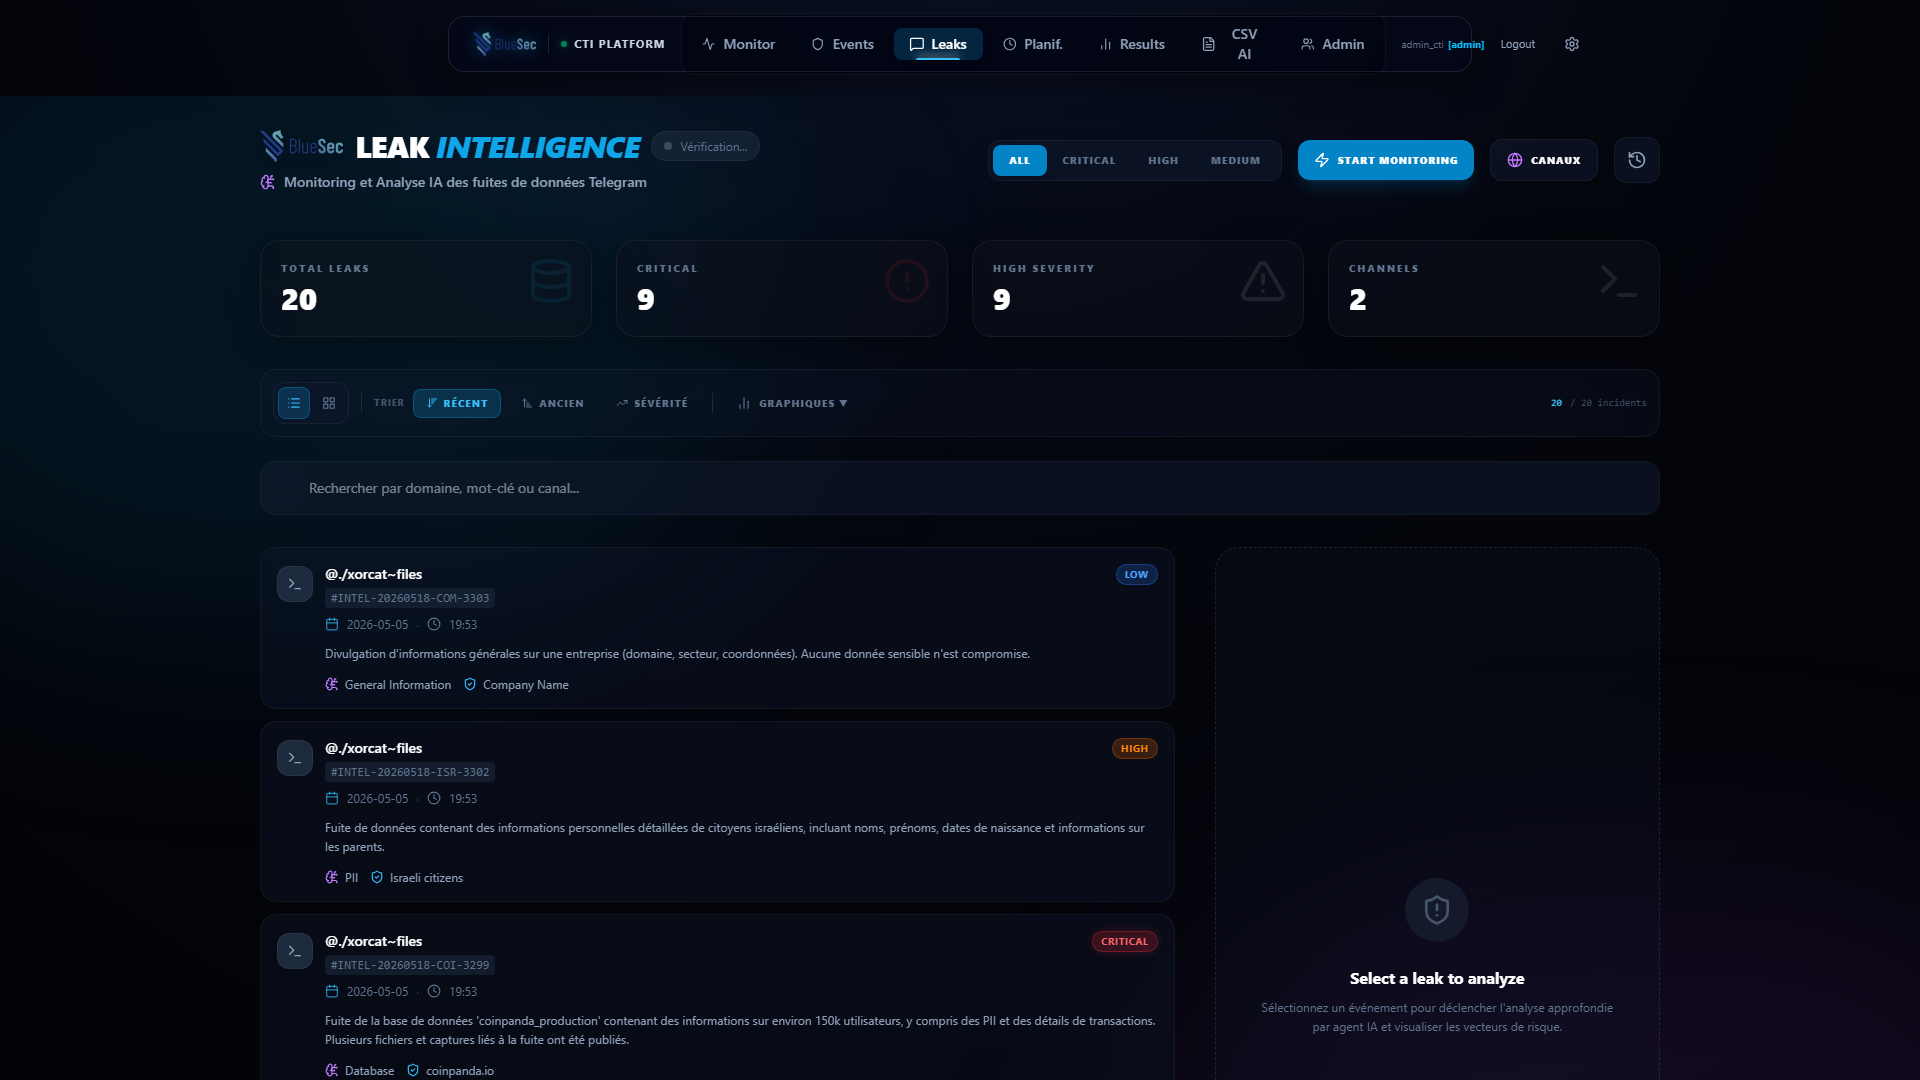
\includegraphics[width=0.9\textwidth]{screenshot/12_page_leaks.png}
    \caption{Liste des fuites de données Telegram identifiées (Threat Leak Intelligence)}
    \label{fig:leaks}
\end{figure}

\section{Implémentation du Backend FastAPI et Frontend React}

L'API REST backend orchestre l'ensemble des requêtes, intégrant un système \textbf{WebSocket} pour le streaming des logs en temps réel. Le frontend, développé en React/Vite, arbore un design Dark Mode "Cyberpunk".

\begin{figure}[H]
    \centering
    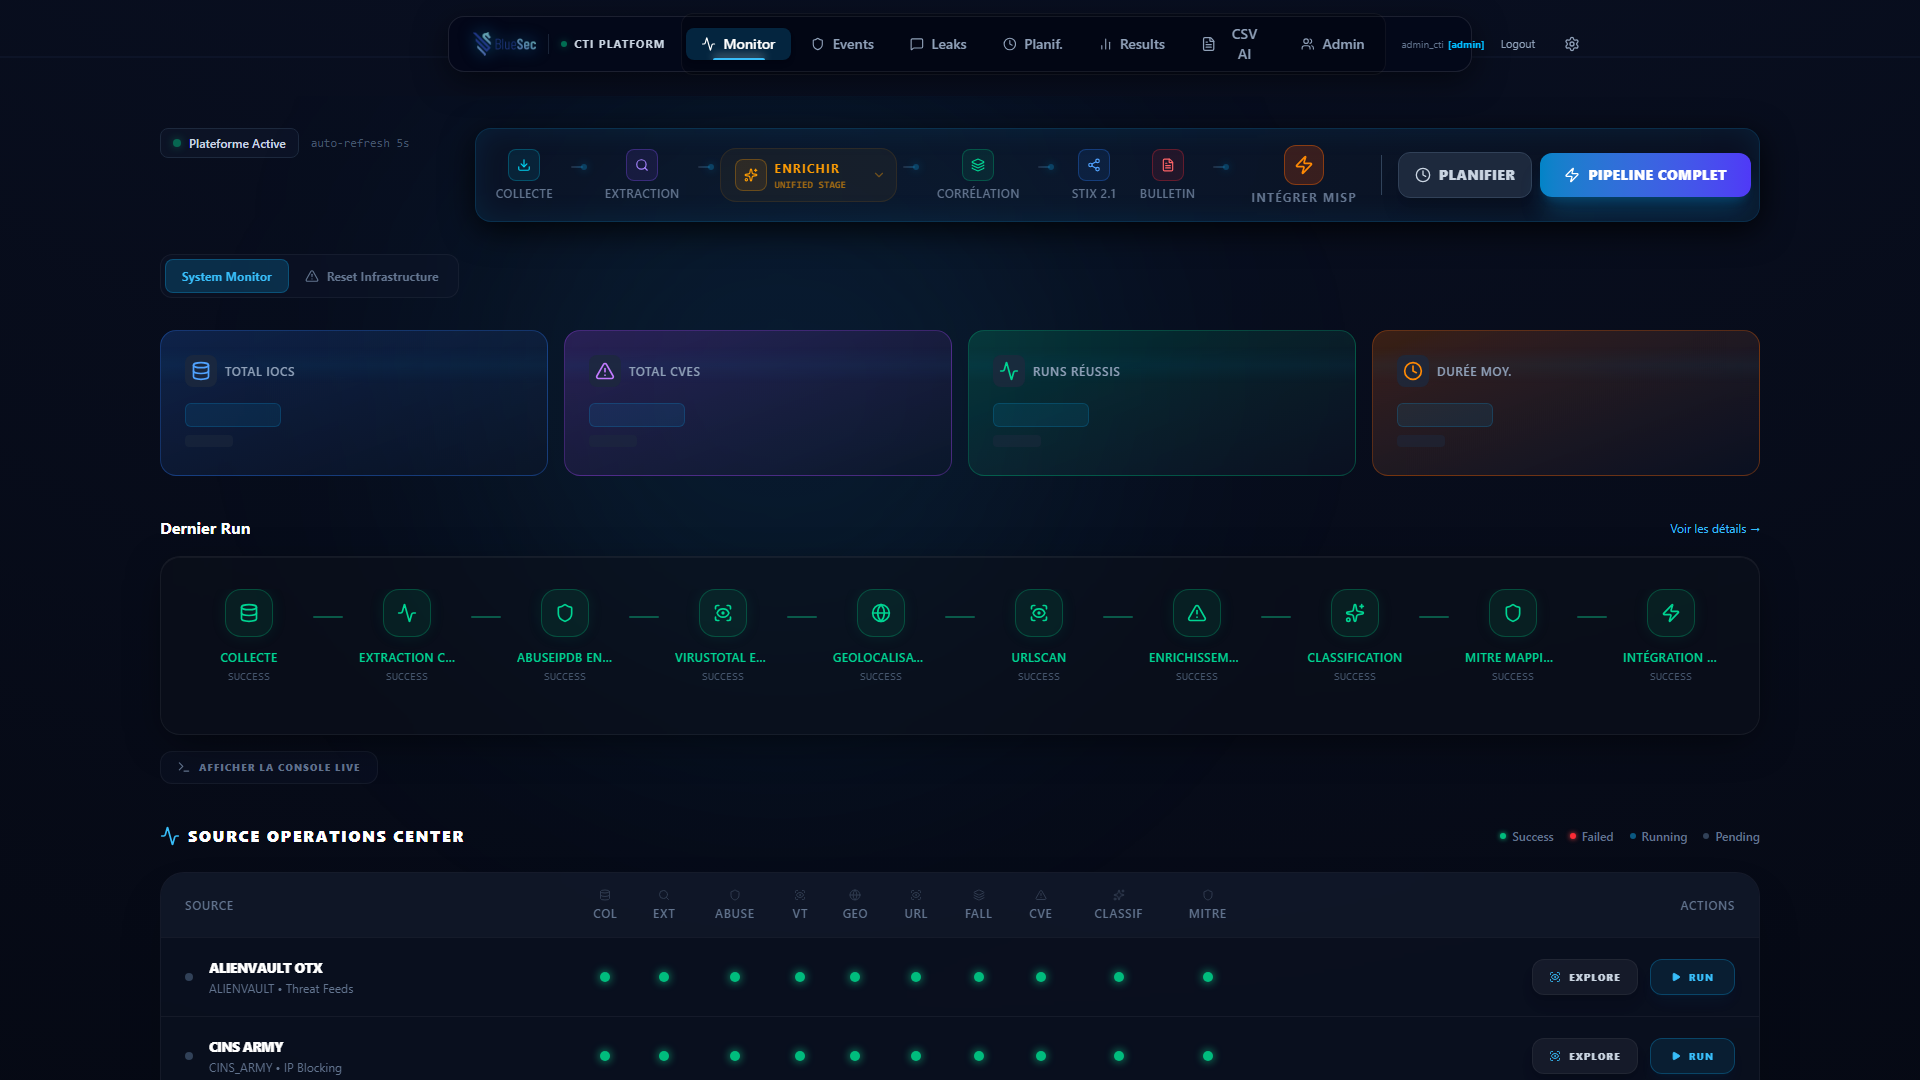
\includegraphics[width=0.9\textwidth]{screenshot/13_carte_geographique.png}
    \caption{Visualisation spatiale des menaces par géolocalisation des adresses IP compromises}
    \label{fig:geo_map}
\end{figure}

\begin{figure}[H]
    \centering
    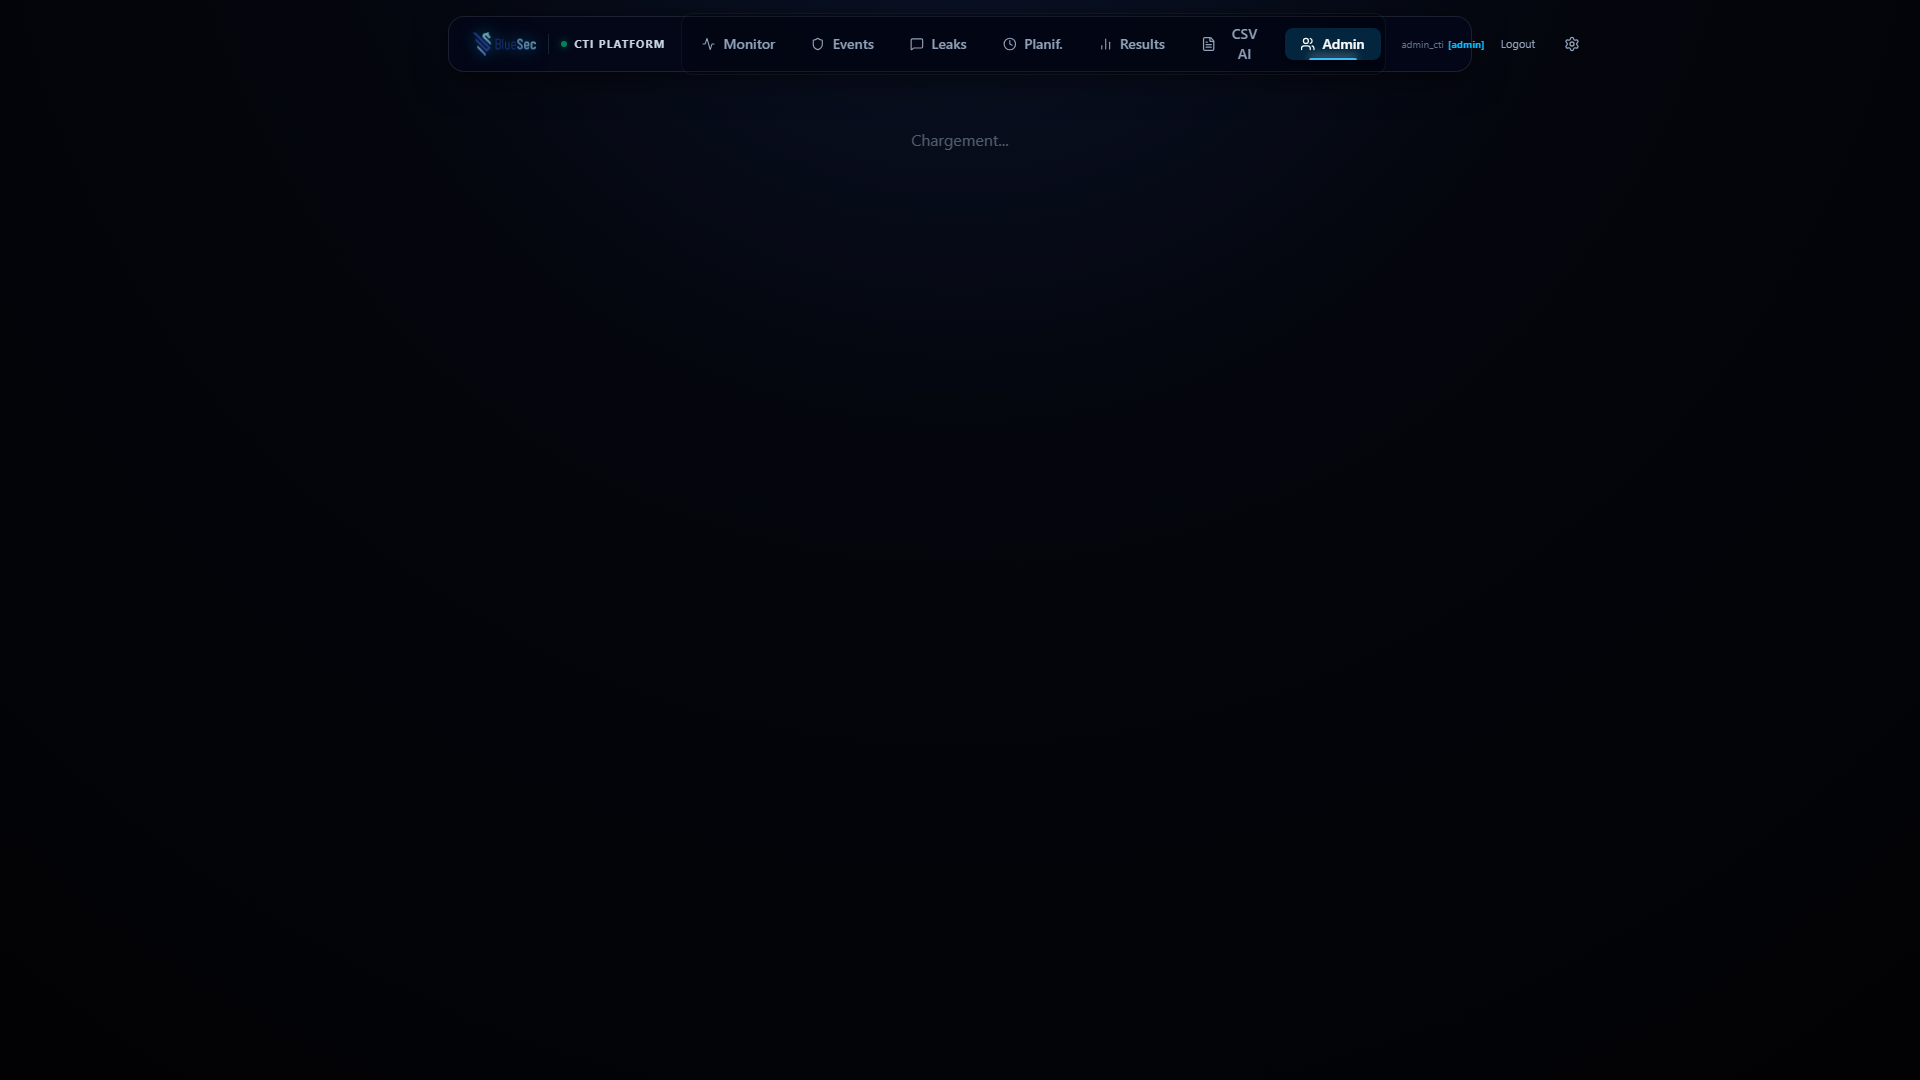
\includegraphics[width=0.9\textwidth]{screenshot/14_panneau_administration.png}
    \caption{Panneau d'administration : Gestion des accès, rôles et clés API OSINT}
    \label{fig:admin_panel}
\end{figure}

\begin{figure}[H]
    \centering
    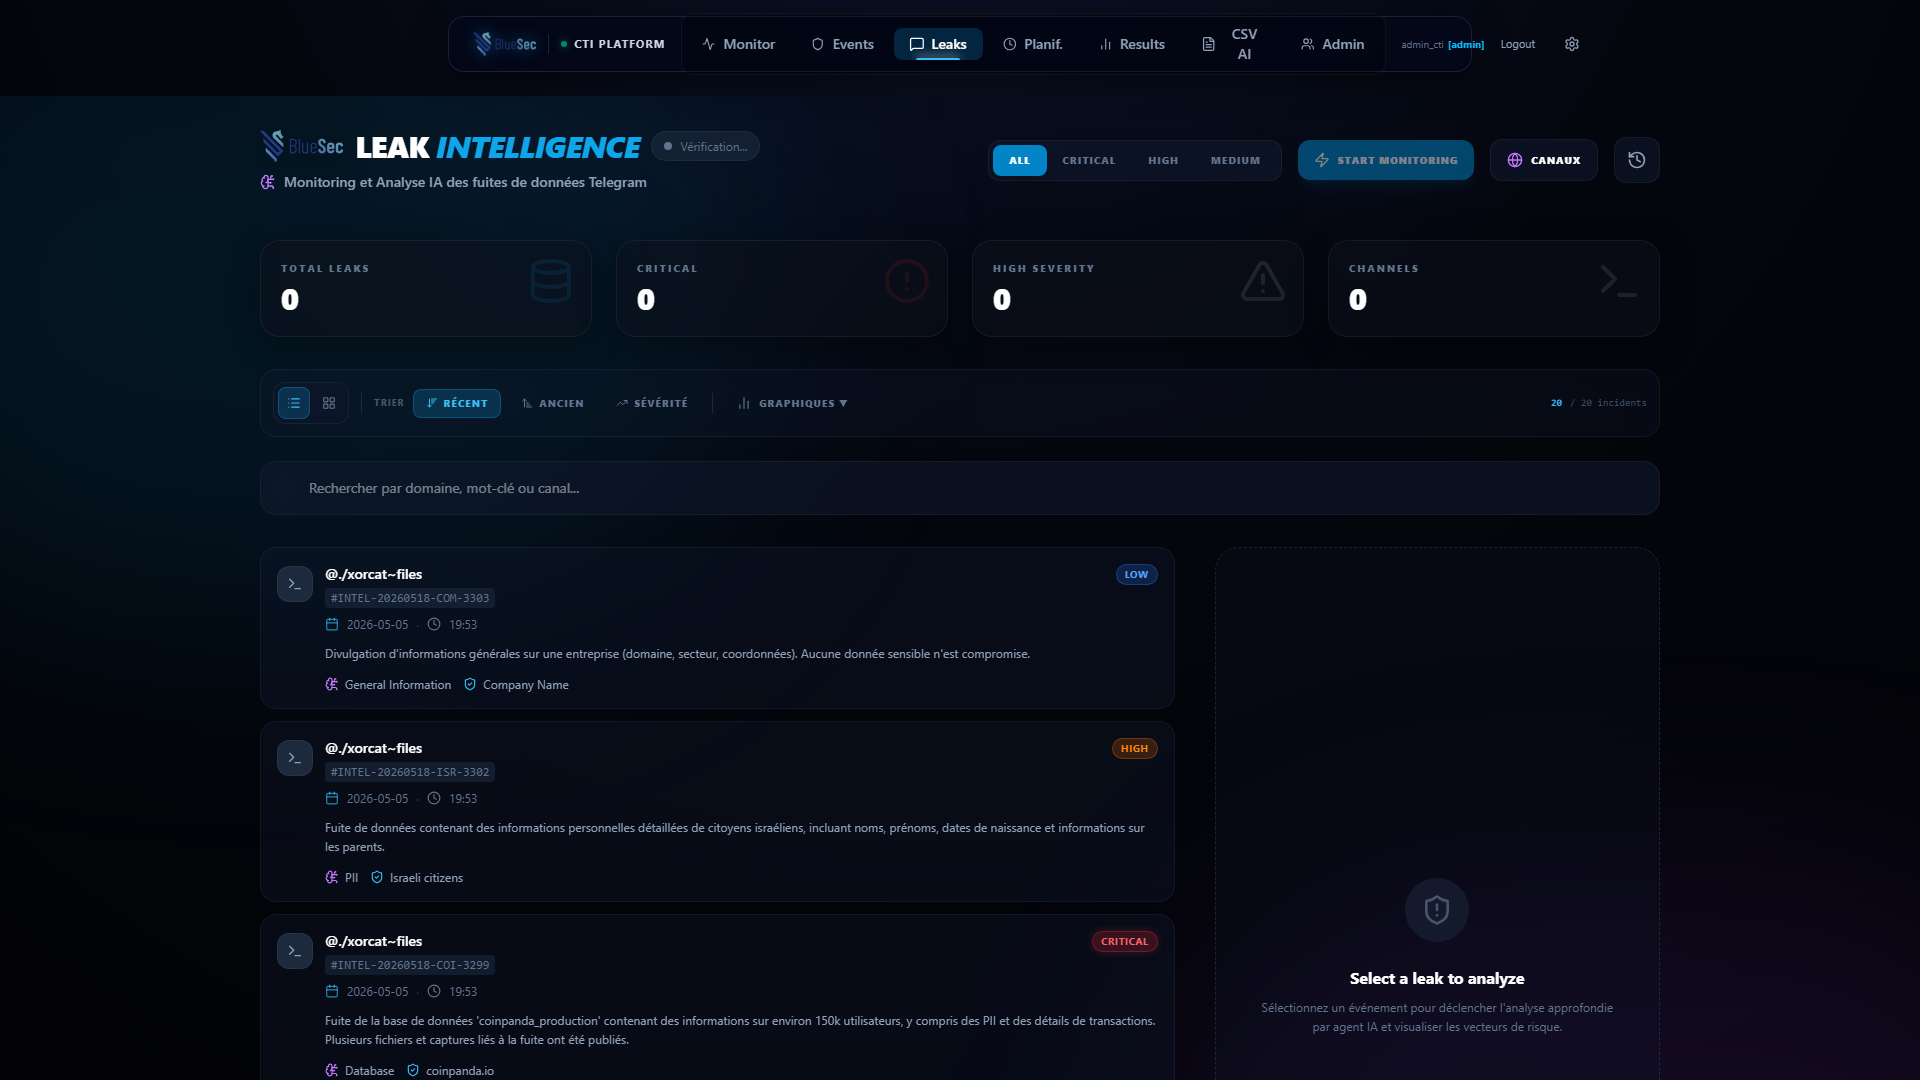
\includegraphics[width=0.9\textwidth]{screenshot/15_bulletin_pdf.png}
    \caption{Extrait d'un bulletin de sécurité SOC PDF généré automatiquement}
    \label{fig:pdf_report}
\end{figure}

\begin{figure}[H]
    \centering
    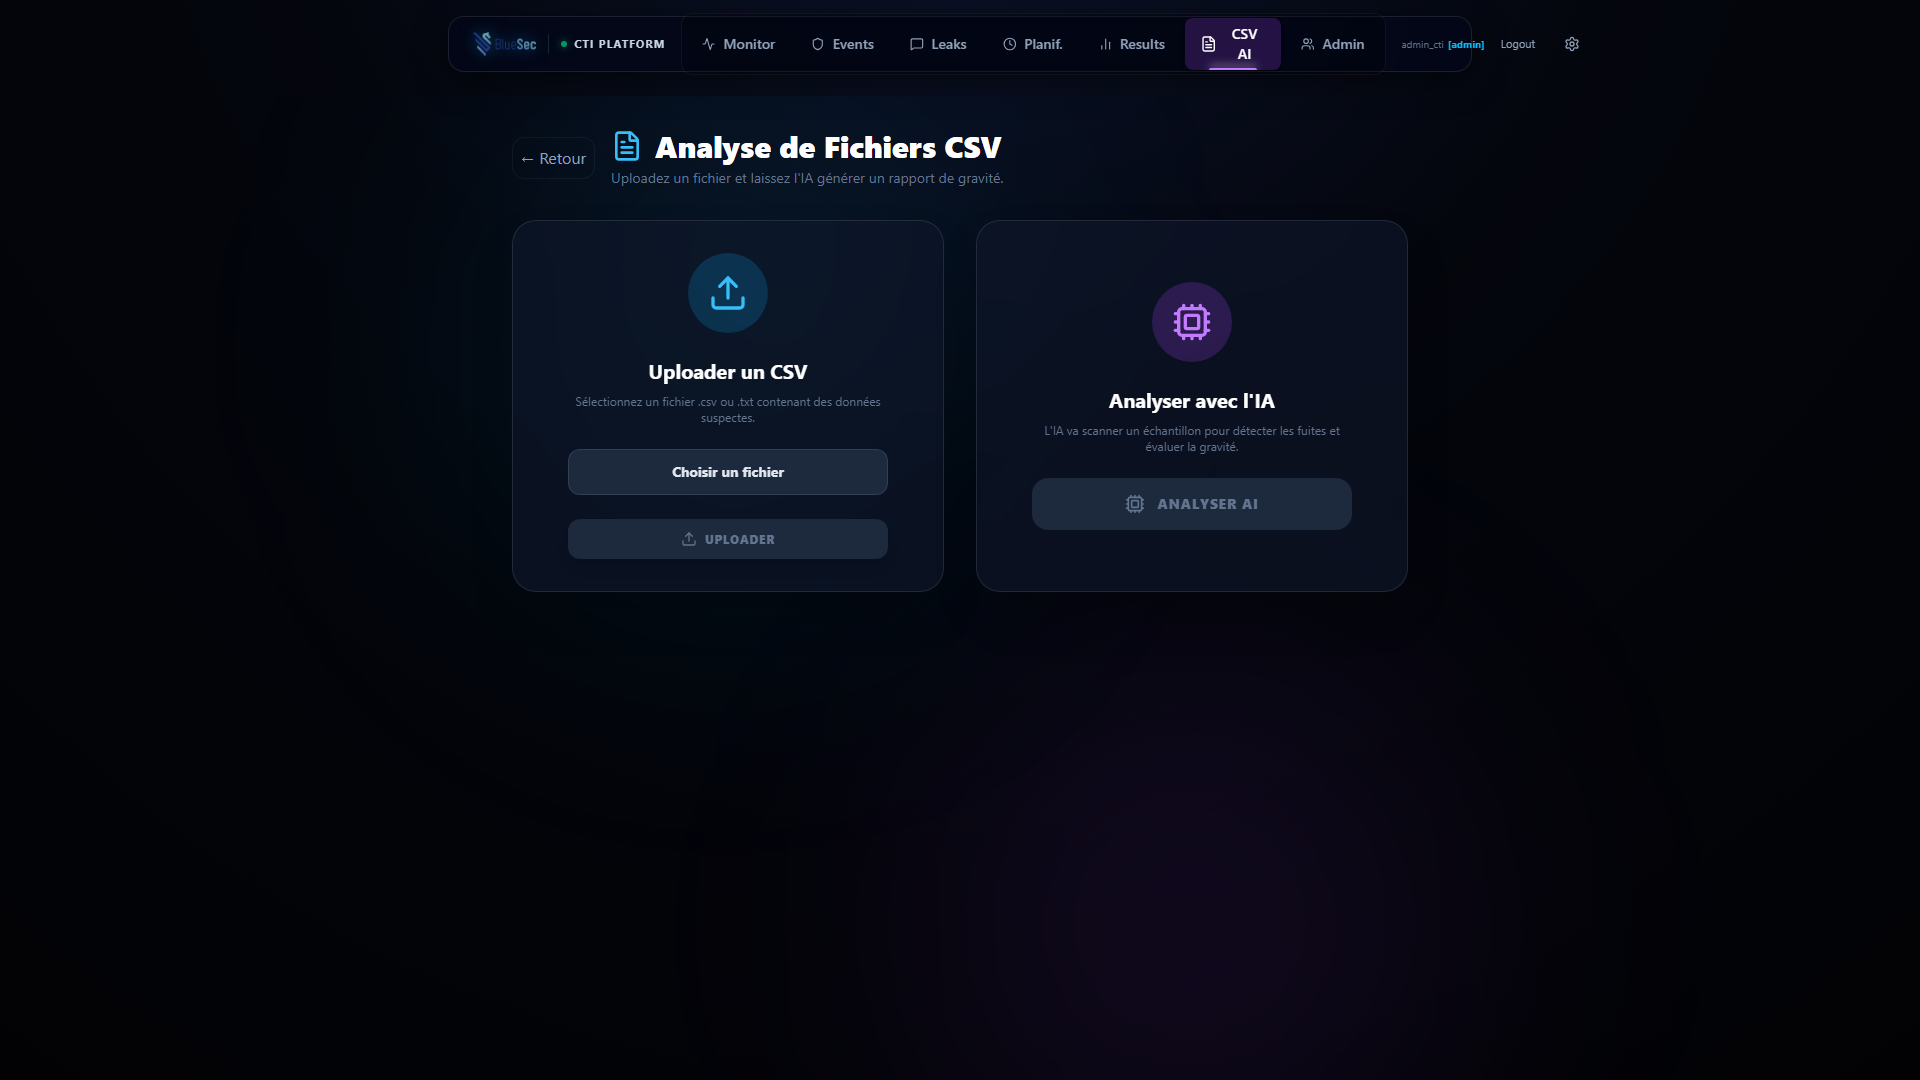
\includegraphics[width=0.9\textwidth]{screenshot/16_analyseur_csv.png}
    \caption{Analyseur CSV intégré au frontend pour l'inspection des bases de données fuitées}
    \label{fig:csv_analyzer}
\end{figure}

\section{Tests et Validation}
Pour garantir la résilience et la fiabilité de l'orchestrateur Cyber-HUD, une batterie de tests a été effectuée.

\subsection{Tests unitaires et d'intégration}
Les modules d'extraction (Regex) et d'enrichissement ont été validés avec des jeux de données de test. L'exécution "end-to-end" du pipeline a confirmé le bon transfert des flux depuis la collecte jusqu'au push MISP.

\subsection{Performances et Métriques}
Le système de géolocalisation local démontre une latence moyenne de moins de 0.5 milliseconde par adresse IP. Le taux de réduction du bruit ("noise cleanup") sur Telegram par le LLM avoisine les 80\%, permettant aux analystes de se concentrer exclusivement sur les fuites avérées.

\section{Conclusion du chapitre}
Ce quatrième chapitre a permis de matérialiser l'architecture conceptuelle proposée. La phase de tests valide la précision de nos extracteurs et la célérité de notre système d'enrichissement. La plateforme Cyber-HUD est fonctionnelle, sécurisée, et prête à être intégrée dans un flux SOC.
